% Tipo de documento
\documentclass[12pt]{article}

% Pacotes
\usepackage{shortvrb}
\usepackage{latexsym}
\usepackage{amsfonts}
%\usepackage[brazil]{babel}
\usepackage[utf8]{inputenc}
\usepackage[pdftex]{graphicx}


% Paginação
\textwidth 17.0cm                     % Largura
\textheight 23.0cm                    % Altura
\addtolength{\oddsidemargin}{-1.6cm}  % Margem esquerda (impar)
\addtolength{\topmargin}{-2.0cm}      % Margem superior

% Estilo dos parágrafos
\sloppy                              % Mais flexível
\setlength{\jot}{13pt}               % Distância entre linhas do eqnarray
\setlength{\parskip}{1ex}            % Distância entre parágrafos
\renewcommand{\baselinestretch}{1.2} % Distância entre linhas

% Comandos customizados
\newcommand{\vet}{\mathbf}                                   % vetor
\newcommand{\ie}{\emph{i.e.}}                                % isto é
\newcommand{\prodint}[2]{\left\langle #1 , #2 \right\rangle} % produto interno
\newcommand{\Fullbox}{{\rule{2.0mm}{2.0mm}}}                 % caixa cheia
\newcommand{\EOS}{\hfill\Box\vspace{-0.2cm}}                 % fim de enunciado
\newcommand{\EOP}{\hfill\Fullbox\vspace{0.2cm}}              % fim de prova
\newcommand{\eps}{\varepsilon}                               % epsilon
\newcommand{\defi}{\: := \: }                                % definição
\newcommand{\del}{\partial}                                  % derivada parcial

%%%%%%%%%%%%%%%%%%%%%%%%%%%%%%%%%%%%%%%%%%%%%%%%%%%%%%%%%%%%%%%%%%%%%%%%%%%%%%%%%%%%%%%%%%%%%%%%%%%%

\begin{document}

\begin{center}
{\large \sc MAC0438 -- Programação Concorrente}

\vspace{0.2cm}

{\large \bf Relatório EP2 -- 22/05/2014}

\vspace{0.5cm}

{\large Daniel Augusto Cortez -- 2960291}

\vspace{0.5cm}
\end{center}    

%%%%%%%%%%%%%%%%%%%%%%%%%%%%%%%%%%%%%%%%%%%%%%%%%%%%%%%%%%%%%%%%%%%%%%%%%%%%%%%%%%%%%%%%%%%%%%%%%%%%

\section{Introdução}

Neste EP implementamos o cálculo da constante de Euler $e$ através da compressão proposta 
em~\cite{brothers04} de sua série de Taylor. A expansão de Taylor para $e$ 
%
\begin{equation} \label{eq:e}
	\sum_{k = 0}^{\infty} \frac{1}{k!} = \frac{1}{0!} + \frac{1}{1!} + \frac{1}{2!} + \cdots 
\end{equation}
%
pode ser comprimida somando $p \geq 1$ termos de uma só vez
%
\[
	\frac{1}{n!} + \frac{1}{(n - 1)!} + \frac{1}{(n - 2)!} + \cdots + \frac{1}{(n - p + 1)!} = 
	\frac{1 + n + n(n - 1) + \cdots + n(n - 1) \cdots (n - p + 2)}{n!} \, ,
\]
%
de onde obtemos (somando de $p$ em $p$):
%
\begin{equation} \label{eq:ec}
	e = \sum_{k = 0}^{\infty} 
		\frac{1 + pk + pk(pk - 1) + \cdots + pk(pk - 1) \cdots (pk - p + 2)}{(pk)!} \, . 
\end{equation}
%
Note que para $p = 1$ recuperamos (\ref{eq:e}). Para $p = 2$, temos
%
\[
	e = \sum_{k = 0}^{\infty} 
		\frac{1 + 2k}{(2k)!} = \frac{1}{0!} + \frac{3}{2!} + \frac{5}{4!} + \cdots \, , 
\]
%
para $p = 3$, temos
%
\begin{equation} \label{eq:p3}
	e = \sum_{k = 0}^{\infty} 
		\frac{1 + (3k)^2}{(3k)!} = \frac{1}{0!} + \frac{10}{3!} + \frac{37}{6!} + \cdots \, , 
\end{equation}
%
e assim por diante. 

Em geral, quanto maior o valor de $p$, maior precisão de obtém com o mesmo número de termos na 
série. Por exemplo, (\ref{eq:p3}) resulta em 78 dígitos corretos com apenas 20 termos.
Além disso, (\ref{eq:p3}) garante melhor estabilidade numérica pelo fato dos numeradores serem 
maiores. É claro que o custo computacional para o cálculo de cada termo também aumenta com $p$. 
Então, existe um {\it tradeoff} entre esses fatores, o qual foi avaliado na implementação proposta.

A soma da série (\ref{eq:ec}) foi feito tanto de forma sequencial quanto paralela. Foram medidos 
os tempos de processamento para diversos valores da precisão requerida, considerando dois critérios 
de parada, bem como diversos valores do parâmetro $p$.

%%%%%%%%%%%%%%%%%%%%%%%%%%%%%%%%%%%%%%%%%%%%%%%%%%%%%%%%%%%%%%%%%%%%%%%%%%%%%%%%%%%%%%%%%%%%%%%%%%%%

\section{Implementação}

Na implementação do cálculo paralelo, foram criadas $n$ threads onde cada uma delas
é responsável pelo cálculo de um termo da série (\ref{eq:p3}) em cada iteração. O valor de $n$ é
definido pelo usuário através do parâmetro \verb|num_threads| passado na linha de comando.

Ao final de uma iteração, a thread deposita o valor do termo calculado no buffer \verb|terms[i]|,
onde $i$ identifica a thread (de $0$ até $n - 1$). Na iteração $j$ a $i$-ésima thread é 
responsável pelo cálculo do termo de número $i + (j - 1) n$. Após depositar o termo calculado, a 
thread aguarda na barreira de sincronização. Após todas as threads chegarem, elas avançam novamente 
para a barreira. Durante esse avanço, a primeira thread ($i = 0$) atualiza o valor de $e$ somando 
todos os termos depositados no buffer e verifica se o critério de parada foi satisfeito.

Existem dois critérios que podem ser passados na linha de comando. O critério \verb|f| indica que 
o cálculo deve parar quando a diferença entre dois valores sucessivos de $e$ (entre iterações) for 
menor do que um parâmetro $\varepsilon$. O critério \verb|m| indica que o cálculo deve parar quando 
qualquer thread calcular um termo menor do que $\varepsilon$. O parâmetro $\varepsilon$ também é 
passado na linha de comando.

Para o cálculo sequencial, utilizamos exatamente a mesma função que realiza o cálculo dos termos no
caso paralelo. A diferença é que ela é chamada sequencialmente e o resultado encontrado é somado a 
$e$ em um loop. Os critérios de parada \verb|f| e \verb|m| coincidem neste caso. 

Na implementação utilizamos a biblioteca GMP para aritmética de múltipla precisão. A manipulação dos
termos da série (\ref{eq:p3}) foi toda realizada com o tipo \verb|mpf_t|, que permite o 
armazenamento de um número de ponto flutuante com precisão limitada apenas pela memória disponível. 

Para evitar o desperdício de memória e otimizar a performance nas operações aritméticas sobre 
\verb|mpf_t|, definimos a precisão padrão do tipo \verb|mpf_t| como sendo 4 vezes o número de casas 
decimais que se deseja no resultado (= o número de casas decimais de $\varepsilon$). Isso porque se 
$t$ é o número de bits da mantissa de \verb|mpf_t|, então $\varepsilon = 2^{-t}$, donde segue que 
$t = - \log_{10} \varepsilon / \log_{10} 2 \approx - 4 \log_{10} \varepsilon$.

Para evitar o cálculo de fatorias repetidos, a variável \verb|max_fat| armazena o maior fatorial 
calculado na iteração anterior. Na iteração corrente, portanto, os produtos dos fatoriais são 
calculados apenas até o valor de \verb|max_fat|. Essa variável é atualizado para a próxima iteração 
com o valor encontrado pela última thread, já que ela é responsável pelo cálculo do maior fatorial.
Apesar de ainda se ter que efetuar diversas multiplicações, especialmente quando o valor de $p$ é 
alto, evitou-se o armazenamento de todos os fatoriais em um vetor que consumiria muita memória. 

O valor do parâmetro $p$ na série (\ref{eq:ec}) foi definido como sendo o número de casas decimais 
que se deseja de precisão dividido por 100. Se esse quociente é menor do que~3, utilizamos o 
valor~3. Assim, utilizamos um valor de $p$ que depende da precisão desejada. Esse critério foi 
definido após alguma experimentação com valores variados de $p$ e $\varepsilon$ na tentativa de se 
minimizar o tempo de processamento. Detalhes sobre esse estudo são apresentados nas próximas seções.  

%%%%%%%%%%%%%%%%%%%%%%%%%%%%%%%%%%%%%%%%%%%%%%%%%%%%%%%%%%%%%%%%%%%%%%%%%%%%%%%%%%%%%%%%%%%%%%%%%%%%

\section{Experimentos}

Os experimentos foram realizados em uma máquina com processador Intel Core~i5 (2.27 GHz) com 4Gb de 
memória RAM, rodando o sistema operacional Linux-Ubuntu 14.04.

O valor de $e$ foi calculado com precisão de 10 até 1.000.000 de casas decimais. Todos os dígitos 
obtidos conferem com os valores apresentados no site \verb|http://www.numberworld.org/digits/E/|.

Apresentamos nos gráficos a seguir valores medidos do tempo de processamento (tempo real, isto é, 
{\it wall clock}) para diversos valores da precisão $\varepsilon$, do número de threads $n$, e 
utilizando ambos os critérios de parada \verb|m| e \verb|f|. Cada tempo foi medido 10 vezes. Os 
valores apresentados correspondem a média e as barras de incerteza, quando presentes, correspondem 
ao desvio-padrão. Todos os testes foram feitos de forma automatizada através das opções \verb|x| e
\verb|y| passadas na linha de comando do programa\footnote{Veja arquivo README para mais 
detalhes.}. Com essas opções nenhum dado de impressão (I/O) é gerado tanto no processamento 
sequencial, quanto no paralelo, permitindo assim uma comparação justa entre os resultados.  

Na Figura~\ref{fig:digitos} fizemos um comparativo entre o desempenho sequencial e paralelo do 
programa, considerando o do tempo de processamento para diversos valores da precisão requerida. O 
parâmetro $p$ da série (\ref{eq:ec}) foi fixado em 10 para esta análise\footnote{Os dados utilizados 
para construção dos gráficos estão disponíveis no arquivo experimentos.xlsx.}. Consideramos ainda os 
critérios de parada \verb|m| e \verb|f|.
%
\begin{figure}[ht]
	\begin{center}
		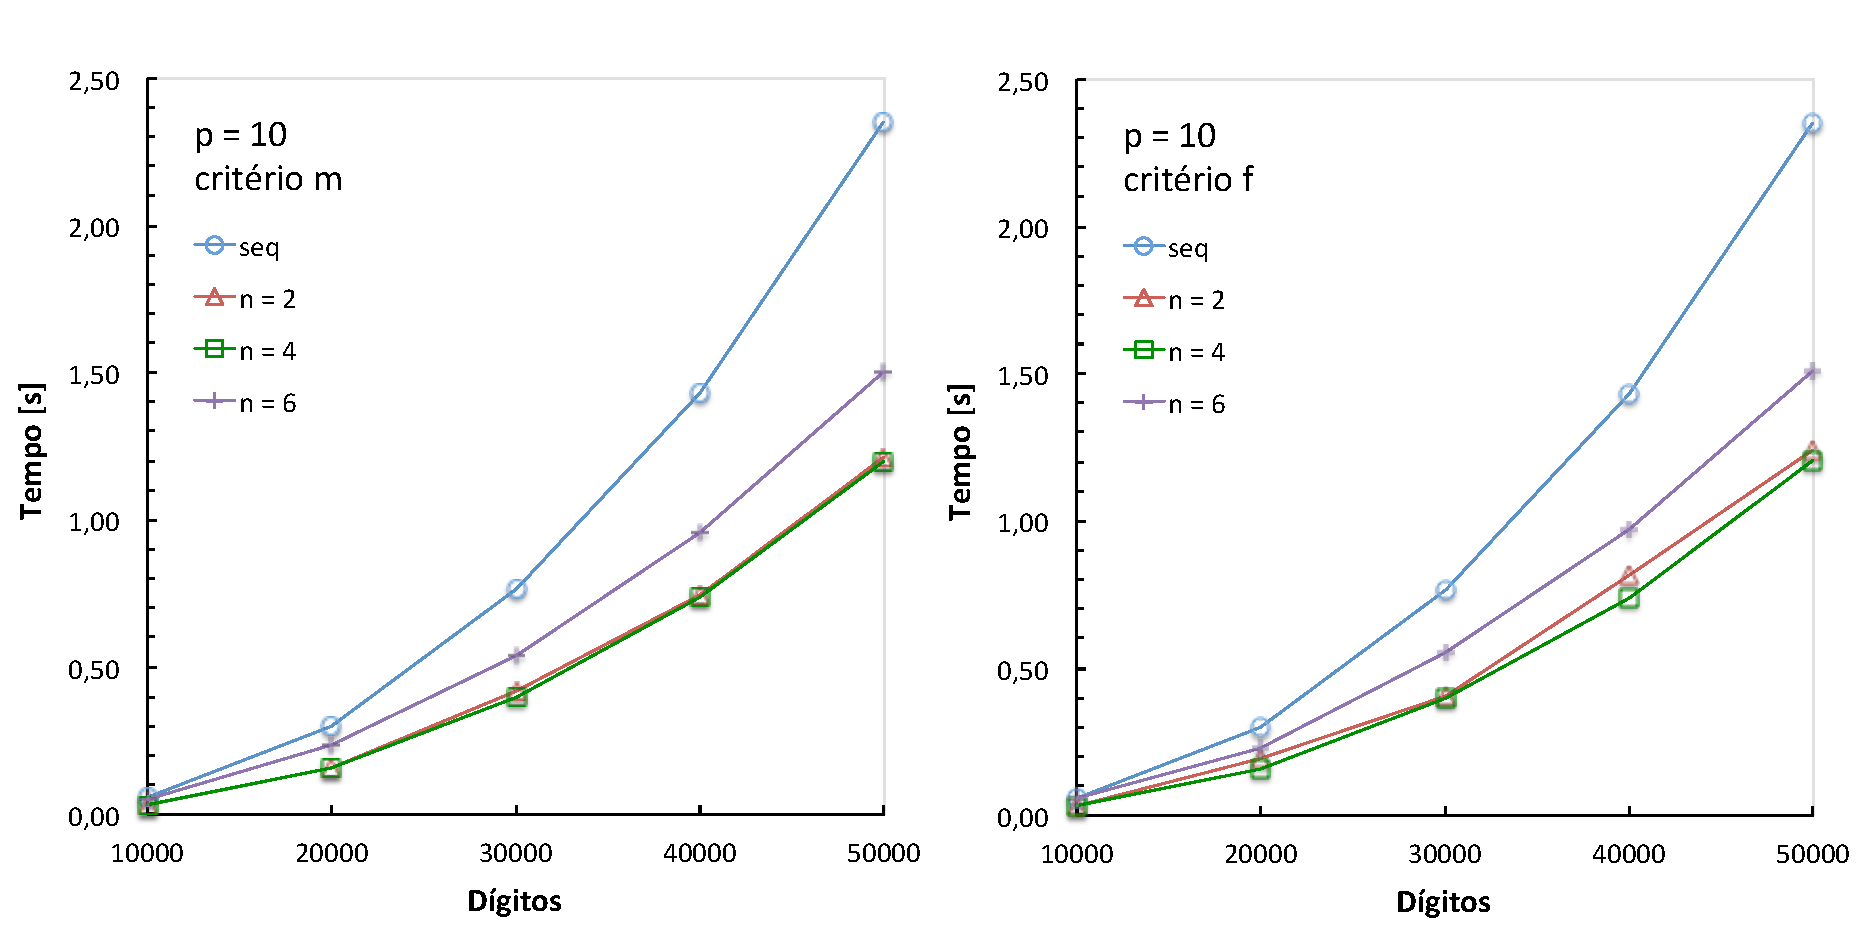
\includegraphics[scale=0.5]{digitos.pdf}
		\caption{Tempo de processamento em função do número de dígitos da precisão desejada. O parâmetro 
		$p$ da série (\ref{eq:ec}) foi fixado com valor 10. No gráfico do lado esquerdo utilizou-se o 
		critério {\bf m} de parada para os casos sequencial (seq) e paralelo ($n = 2, 4, 6$ threads). 
		No gráfico do lado direito utilizou-se o critério {\bf f}. As barras de incerteza nos pontos 
		foram removidas por serem muito pequenas para a escala da figura.}
		\label{fig:digitos} 
	\end{center}
\end{figure}

Na Figura~\ref{fig:p} analisamos o tempo de processamento dos algoritmos sequencial e paralelo, 
variando o parâmetro $p$ da série (\ref{eq:ec}). Foram analisadas duas situações de precisão 
requerida: 10.000 e 50.000 dígitos. Para o processamento paralelo, considerou-se apenas $n = 4$ 
threads, correspondente ao número de núcleos do computador onde se realizou os testes.
%
\begin{figure}[ht]
	\begin{center}
		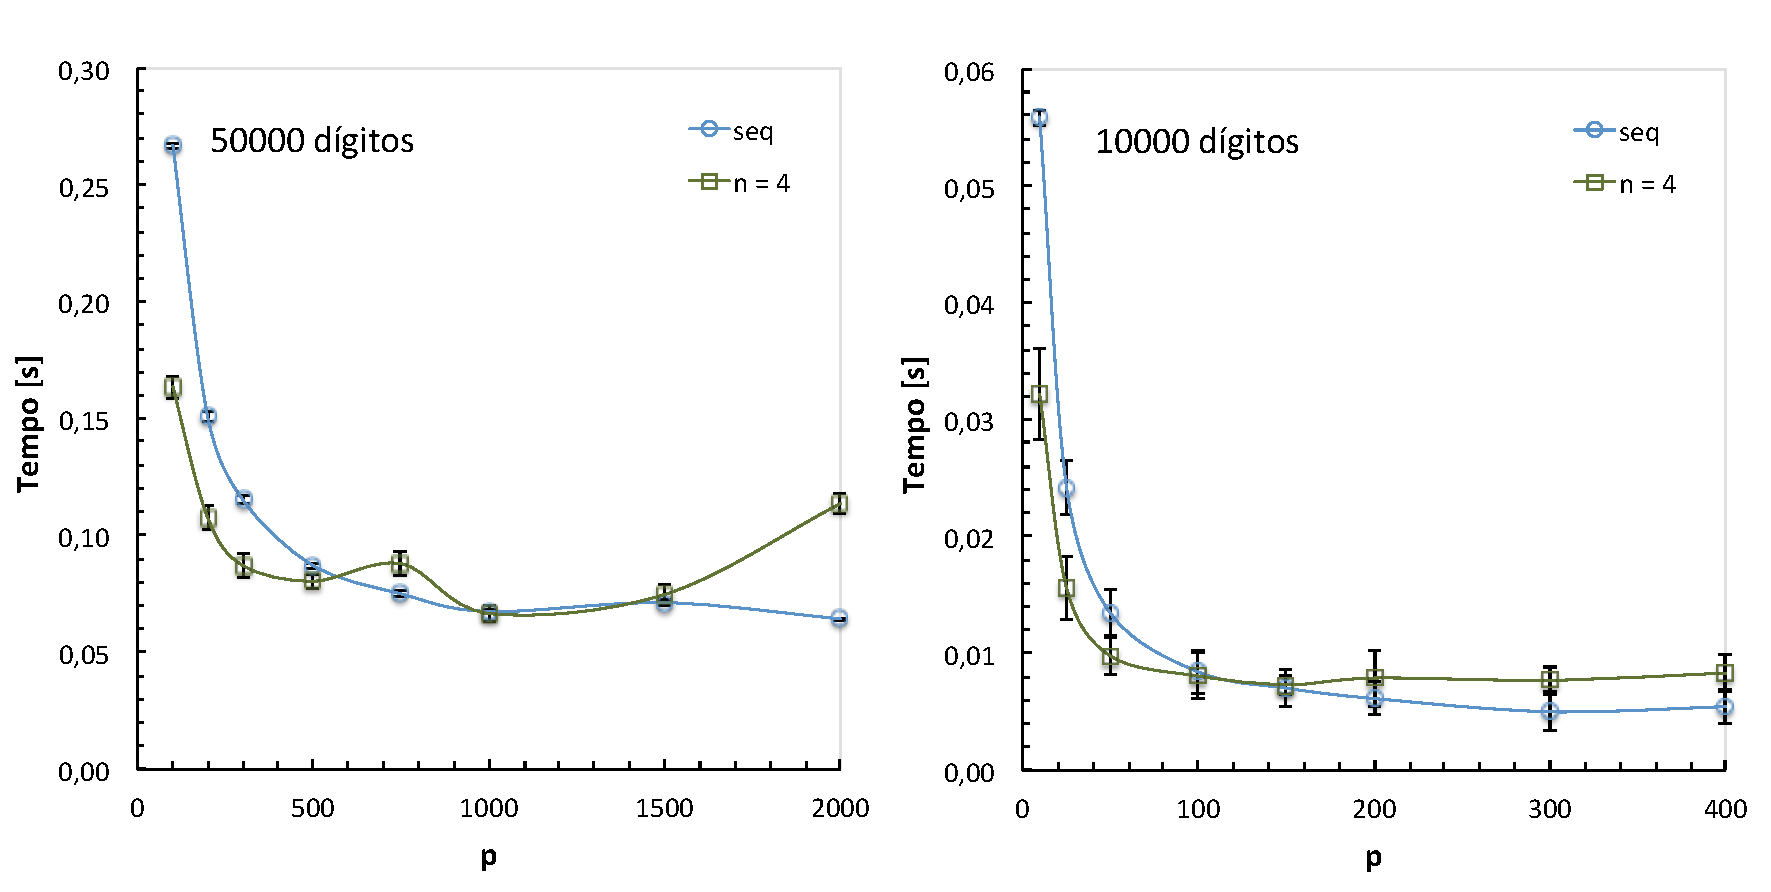
\includegraphics[scale=0.5]{p.pdf}
		\caption{Tempo de processamento em função do parâmetro $p$ da série (\ref{eq:ec}). No gráfico do 
		lado esquerdo foram considerados 50000 dígitos de precisão, tanto no cálculo sequencial (seq), 
		como no cálculo paralelo ($n = 4$ threads). No gráfico do lado direito foram considerados 10000 
		dígitos de precisão.}
		\label{fig:p} 
	\end{center}
\end{figure}

%%%%%%%%%%%%%%%%%%%%%%%%%%%%%%%%%%%%%%%%%%%%%%%%%%%%%%%%%%%%%%%%%%%%%%%%%%%%%%%%%%%%%%%%%%%%%%%%%%%%

\section{Conclusões}

Os gráficos da Figura~\ref{fig:digitos} indicam claramente um desempenho aproximadamente duas vezes 
superior da versão paralela do programa, com relação à versão sequencial (considerando o valor de 
$p$ fixo e pequeno). A curva de melhor desempenho corresponde a $n = 4$, justamente igual ao número 
de núcleos do computador onde se realizaram os testes. Muito próxima a ela está a curva com $n = 2$. 
Já para $n = 6$, o desempenho piora, mas não chega a ser pior do que o caso sequencial. Os 
experimentos confirmam o comportamento esperado. 

Ambas as implementações apresentam bom desepenho, calculando 50.000 dígitos de $e$ em um tempo da 
ordem de 1~segundo. Para o cálculo de $e$ com 1.000.000 de dígitos, o programa leva da ordem de 
15~segundo para finalizar.

Os gráficos da Figura~\ref{fig:p} foram utilizados para estimar o valor do parâmetro $p$ que 
proporciona o melhor desempenho em função da precisão pretendida. Claramente o desempenho melhora à 
medida que aumentamos $p$ até atingirmos um valor em que ele se torna praticamente constante. Aliás, 
para $p$ suficientemente grande, o desempenho da implementação sequencial é melhor do que da 
paralela. Como pode ser observado nas curvas, o {\it menor} valor de $p$ tal que o desempenho é 
maximizado, tanto para a versão sequencial, quanto para paralela, é dado aproximadamente pelo valor 
da precisão dividido por 100 (500 para 50.000 dígitos e 100 para 10.000 dígitos). Essa regra é 
utilizada por padrão na implementação do programa quando não se especifica o valor a ser utilizado 
para $p$ na linha de comando. 

É interessante observar que o desempenho da versão paralela é superado pela versão sequencial quando
$p$ é suficientemente grande. Na Figura~(\ref{fig:seq}) apresentamos uma fotografia do monitor do 
sistema do Ubuntu durante a execução sequencial do programa, utilizando um valor grande de $p$ para
o cálculo de $e$ com 1.000.000 de dígitos. Observe que a CPU escolhida para rodar a thread apresenta 
100\% de utilização enquanto as demais são pouco utilizadas.  
%
\begin{figure}[ht]
	\begin{center}
		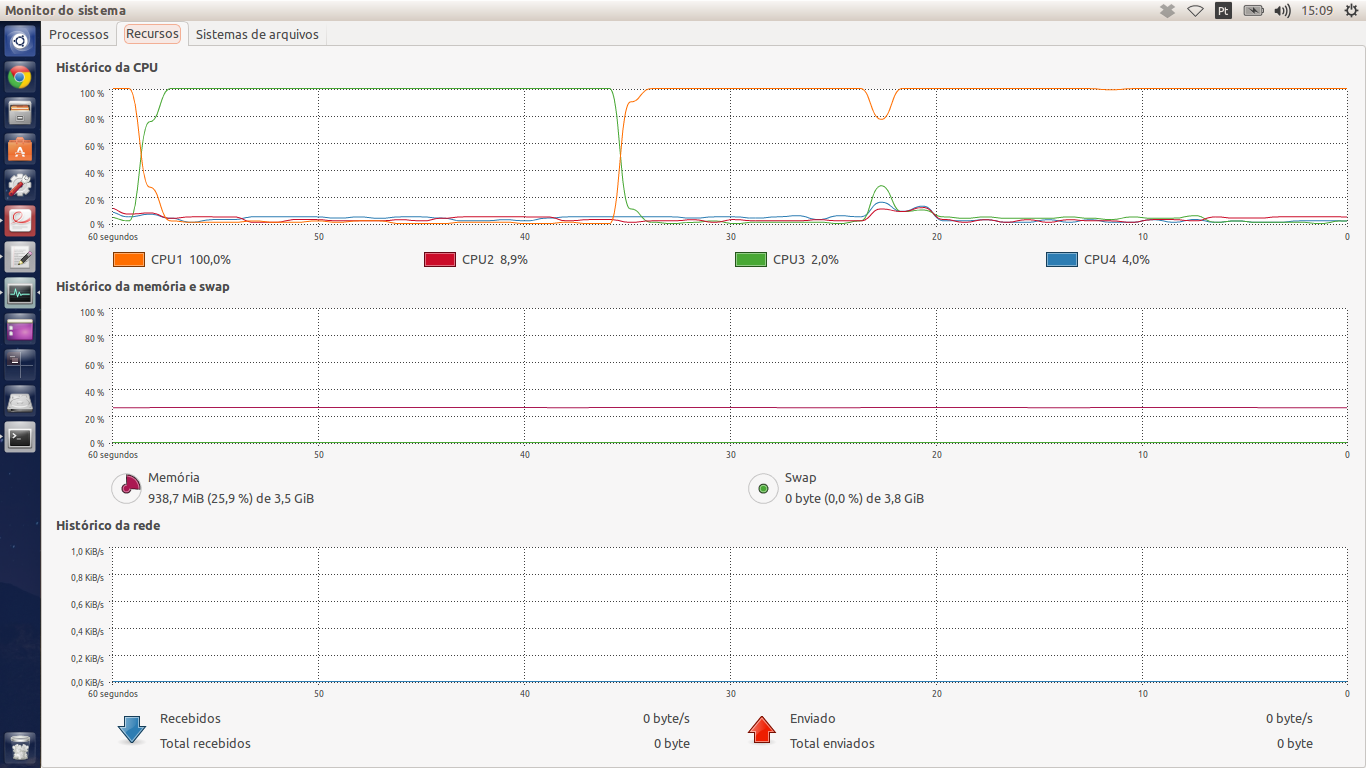
\includegraphics[scale=0.275]{sequencial.png}
		\caption{Histórico da CPU durante execução sequecial do programa. Observe a utilização de 100\%
		da CPU1 enquanto as demais estão praticamente ociosas. Observe também a provável comutação da 
		thread executando na CPU3 para a CPU1 no tempo 35 segundos.}
		\label{fig:seq} 
	\end{center}
\end{figure}

Na Figura~\ref{fig:par1} apresentamos uma fotografia do monitor do sistema em condições análogas 
às da Figura~\ref{fig:seq}, mas agora considerando a execução paralela do programa. Note como 
existe uma grande oscilação na utilização das CPUs. Isso provavelmente ocorre pelo fato de que para
$p$ grande, do jeito como foi implementado o cálculo do fatorial utilizando o maior valor calculado 
na iteração anterior, a última thread tem que calcular um número muito maior de produtos do que a 
primeira, logo ela chega bem depois na barreira de sincronização. Isso fica evidente ao se rodar o
programa com a opção de debug \verb|d|. Note como as threads chegam sempre em ordem na barreira:

\begin{small}
\begin{verbatim}
	[Thread 0 chegou na barreira na iteração 1]
	[Thread 1 chegou na barreira na iteração 1]	
	[Thread 2 chegou na barreira na iteração 1]
	[Thread 3 chegou na barreira na iteração 1]

	[Thread 0 chegou na barreira na iteração 2]
	[Thread 1 chegou na barreira na iteração 2]
	[Thread 2 chegou na barreira na iteração 2]
	[Thread 3 chegou na barreira na iteração 2]

	[Thread 0 chegou na barreira na iteração 3]
	[Thread 1 chegou na barreira na iteração 3]
	[Thread 2 chegou na barreira na iteração 3]
	[Thread 3 chegou na barreira na iteração 3]
\end{verbatim}
\end{small}

Dessa forma, o desempenho do programa fica muito parecido com o desempenho sequencial, com a 
desvantagem de ocorrer muito mais trocas de contexto, e com os problemas de atualização do cache. 
Isso explica a perda de performance da implmentação paralela para $p$ grande.

\begin{figure}[ht]
	\begin{center}
		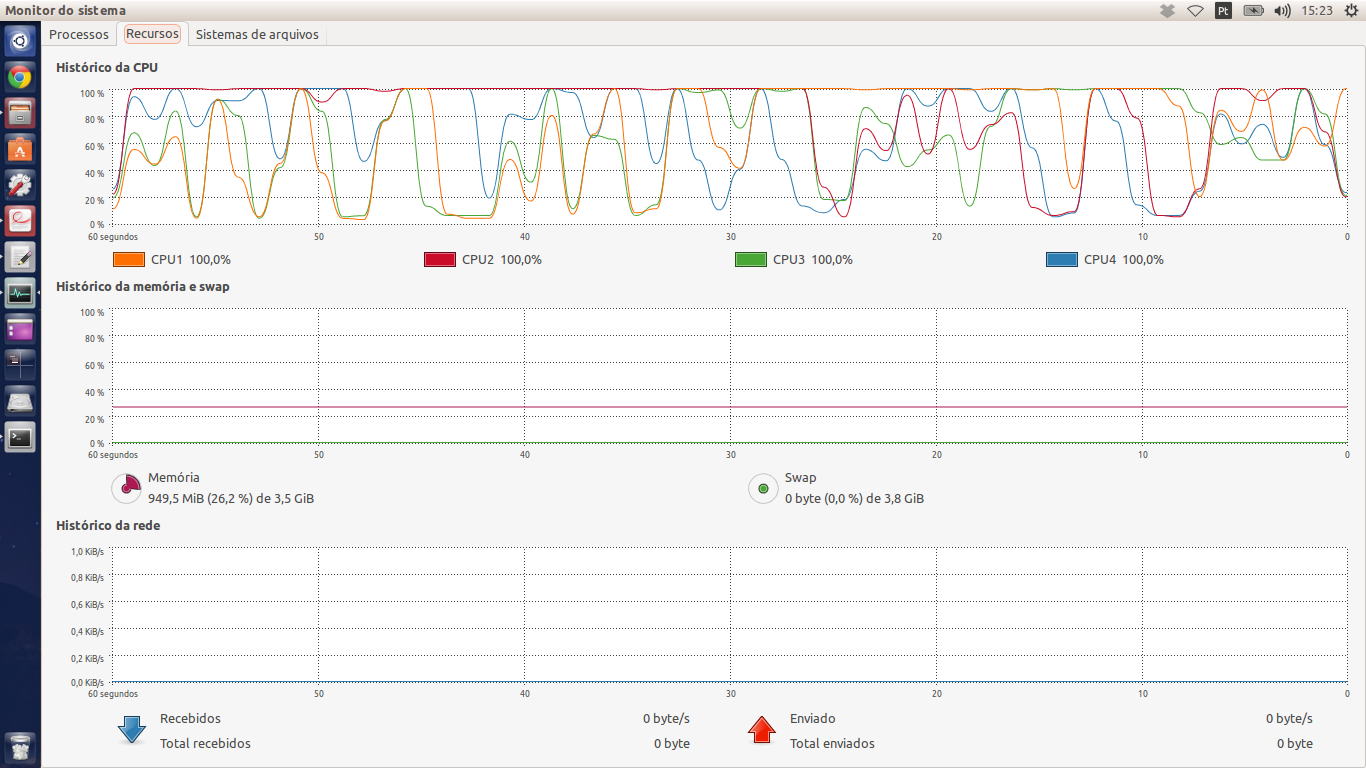
\includegraphics[scale=0.275]{paralela1.png}
		\caption{Histórico da CPU durante execução paralela do programa para $p$ grande. Observe a 
		utilização oscilante das 4 CPUs. Este é o caso em que o desempenho paralelo é inferior ao 
		sequencial.}
		\label{fig:par1} 
	\end{center}
\end{figure}

Por outro lado, para $p$ pequeno, o problema com o cálculo dos fatoriais não é tão sensível. Todas
as threads tem carga de trabalho parecida, e portanto, chegam na barreira de forma mais ou menos 
concorrente, não havendo nenhum gargalo de espera. Isso é evidente ao se observar a 
Figura~\ref{fig:par2}. Ela foi gerda de forma similar à Figura~\ref{fig:par1}, mas considerando um
valor pequeno de $p$. Observe como todas as CPUs ficam 100\% utilizadas praticamente o tempo todo.
Essa situação leva ao ganho de performance da implementação paralela sobre a sequencial, evidenciado
nos gráficos da Figura~\ref{fig:digitos}.

\begin{figure}[ht]
	\begin{center}
		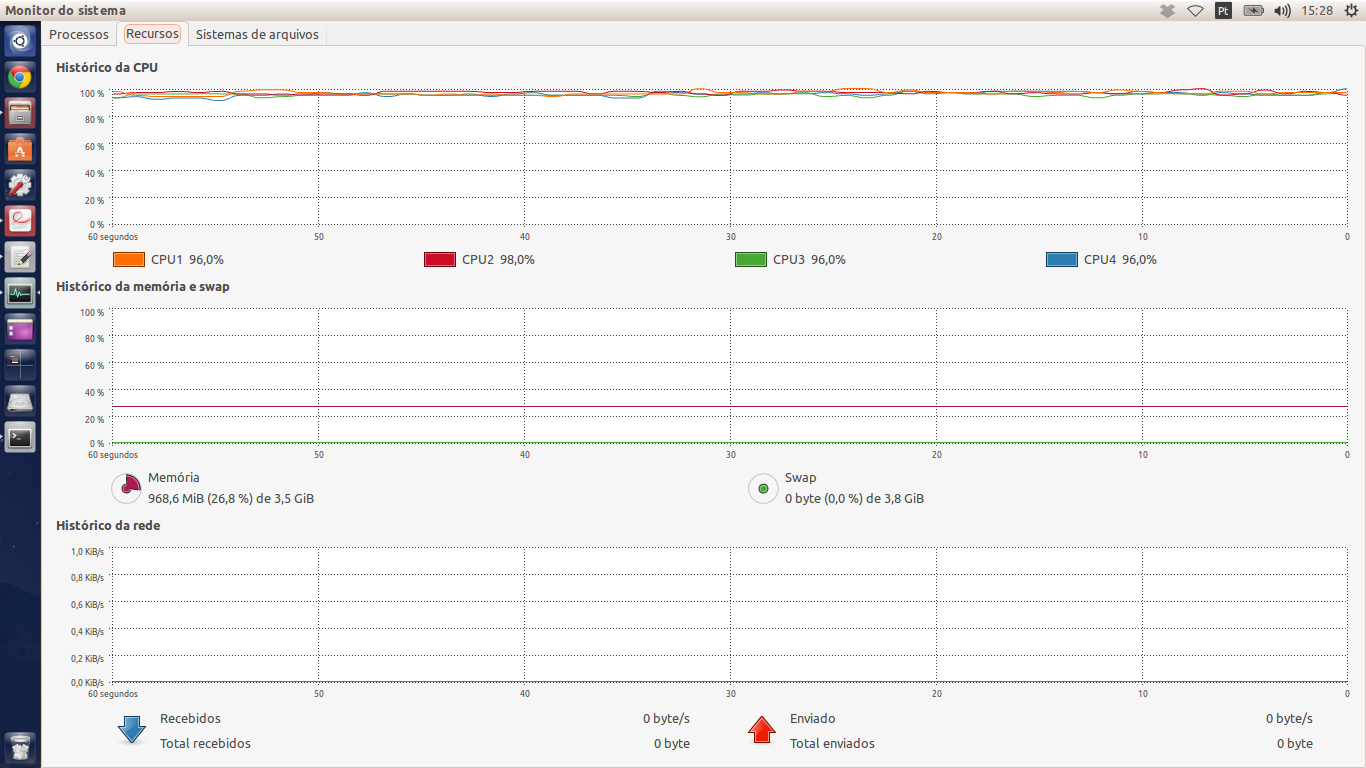
\includegraphics[scale=0.275]{paralela2.png}
		\caption{Histórico da CPU durante execução paralela do programa para $p$ pequeno. Observe a 
		utilização praticamente constante de 100\% das 4 CPUs. Este é o caso em que o desempenho 
		paralelo é supeior ao sequencial.}
		\label{fig:par2} 
	\end{center}
\end{figure}

%%%%%%%%%%%%%%%%%%%%%%%%%%%%%%%%%%%%%%%%%%%%%%%%%%%%%%%%%%%%%%%%%%%%%%%%%%%%%%%%%%%%%%%%%%%%%%%%%%%%

\begin{thebibliography}{9}

\bibitem{brothers04} H.~J.~Brothers. {\it Improving the convergence of Newton's series approximation 
for $e$}. The College Mathematics Journal, {\bf 35}, No.~1, 2004 (34-39).

\end{thebibliography}

%%%%%%%%%%%%%%%%%%%%%%%%%%%%%%%%%%%%%%%%%%%%%%%%%%%%%%%%%%%%%%%%%%%%%%%%%%%%%%%%%%%%%%%%%%%%%%%%%%%%

\end{document}
